\fancyhead[LO, RE]{Création d'annotations}

Dans l'intérêt d'accomplir une analyse plus approfondie que celle que nous venons de réaliser, nous devons nous intéresser au cœur du texte. Notre attention se portera principalement sur son lexique juridique, réduisant de ce fait le champ d'analyse et permettant d'être en lien avec la finalité du projet MetaLEX\index{Projet MetaLEX}, le dictionnaire métalexicographique composé de termes juridiques. L'objectif consiste à établir une liste contenant des termes juridiques extraits du texte de Beccaria\index{Beccaria, marquis de}, que nous pourrons ensuite manipuler pour en faire des annotations à insérer dans le texte, afin de rendre possible ultérieurement une exploitation de ces données. Avant d'atteindre ce résultat, il est cependant nécessaire d'établir la liste de ces termes juridiques en prenant en compte toutes les langues du corpus pour ensuite amplifier cette liste et la transformer de manière à annoter le texte et pouvoir tirer parti de ces annotations.

\section{Déterminer les termes clés~: création des listes adéquates et compatibles pour l'analyse}
L'étape primordiale pour pouvoir réaliser le travail d'annotations est la réalisation de la liste de termes clés juridiques ou liés au juridique qui servira ensuite à nos analyses.

Cette liste a déjà été en partie réalisée par une des membres du projet, Claudine Moulin, à l'occasion du séminaire de février sur \og~Les mots du droit~\fg{}. Elle prend en compte trois des quatre langues de nos éditions et donne les équivalents des termes pour chacune d'entre elles. Si cette liste est une base pour l'élaboration de notre dictionnaire de termes clés, elle possède tout de même quelques lacunes qui impactent son exploitation.

\subsection{Une liste de termes noyaux initialement établie}
Pour établir sa liste de termes, Claudine Moulin s'est basée sur la version française du \emph{Traité des délits et des peines}\index{Traite des delits et des peines@Traité des délits et des peines} traduit par Philippe Audegean en 2009\footcite{beccaria_audegean_2009} et en a extrait les termes qui étaient considérés comme appartenant au lexique juridique à étudier. 
\begin{figure}[H]
    \centering
    \fbox{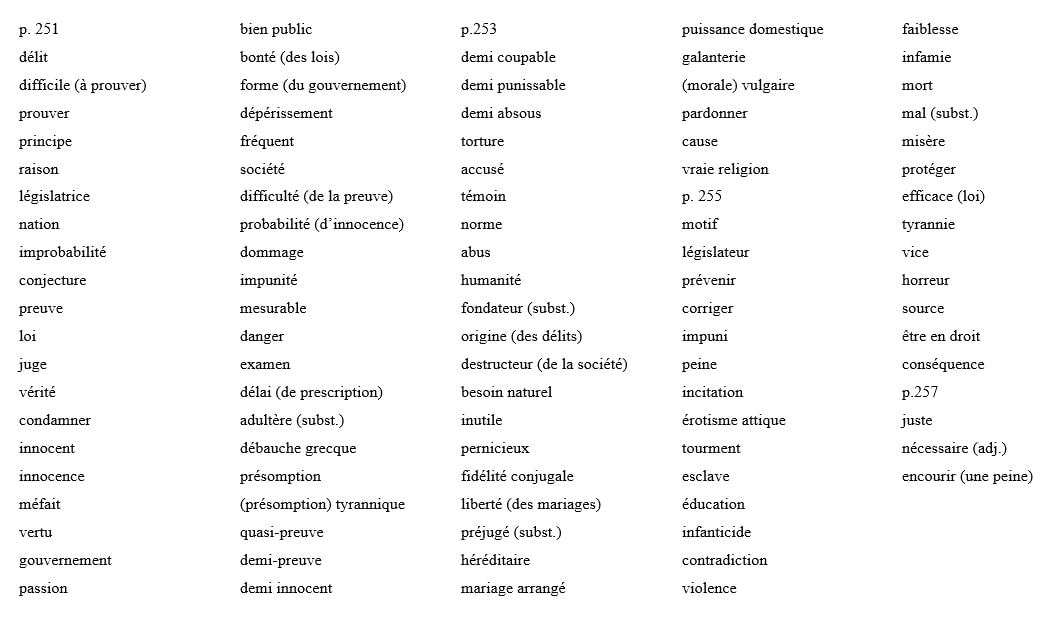
\includegraphics[width=16cm]{Partie3/images/chap2/termes_cles1.jpg}}
    \caption{Liste des termes clés choisis en français du chapitre 30/31/36 du \emph{Traité}\index{Traite des delits et des peines@Traité des délits et des peines} de Beccaria\index{Beccaria, marquis de}}
    \label{fig:termes_cles1}
\end{figure}
Ensuite, les mots relevés dans le texte ont été transformés pour conserver seulement leur lemme (c'est-à-dire leur version au masculin singulier, à l'infinitif, etc., en fonction de la catégorie grammaticale) pour que cela soit plus adéquat pour une exploitation future. L'action suivante a consisté à aller rechercher les équivalents dans les autres langues, en prenant pour appui la version de 1766 de Beccaria\index{Beccaria, marquis de} pour l'italien et une version contemporaine de 1966 pour l'allemand (l'anglais n'a pas été traité dans son tableau). En conséquence, le résultat obtenu est une liste multilingue contenant tous les termes considérés comme pertinents pour nos futures analyses.

Cette liste compte un peu moins d'une centaine de mots ou expressions lexicales relatifs au droit et au sujet traité dans le chapitre 30/31/36 pris en compte pour l'établissement de cette liste.
\begin{figure}[H]
    \centering
    \fbox{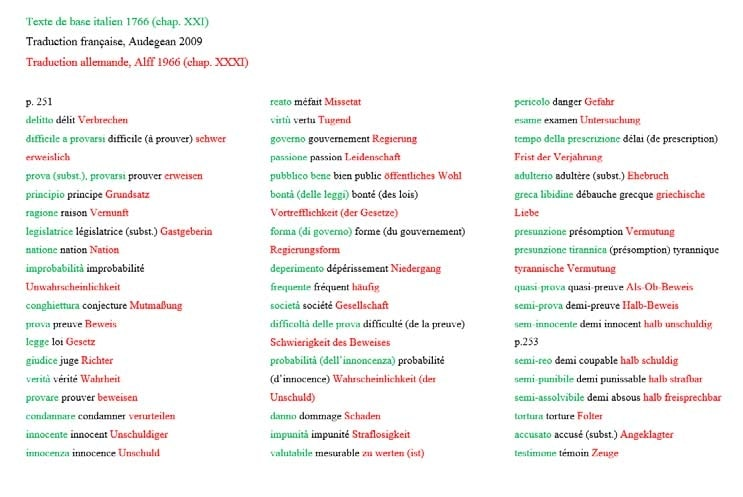
\includegraphics[width=16cm]{Partie3/images/chap2/termes_cles2.jpg}}
    \caption{Première partie de la liste de termes clés établie par Claudine Moulin}
    \label{fig:termes_cles2}
\end{figure}

\subsection{Comment perfectionner la liste~: séries de modifications à apporter}
La liste de termes noyaux nécessite des changements car elle ne correspond pas tout à fait à ce que nous rechercherons. Si l'édition modèle utilisée pour l'italien fonctionne bien car elle date de 1766, les deux autres versions posent problèmes car l'allemand et le français sont issus d'éditions contemporaines. Il est donc nécessaire de repartir vers les éditions d'avant 1800 pour chercher les expressions ou mots avec une correspondance exacte dans le fond du texte et intégrer dans la liste l'anglais, qui fait également partie de notre étude.

\subsubsection{Choisir une édition modèle pour chaque langue}
Le meilleur moyen de récupérer des expressions correctes est de choisir une édition modèle pour chaque langue et d'effectuer une lecture attentive du texte~; dans mon cas, j'ai choisi de faire une lecture phrase par phrase entre les différentes langues pour trouver exactement le terme choisi par les traducteurs dans les autres langues.

Ainsi, en italien, l'édition modèle est celle de 1766 (it5)\footcite{it5}, qui contient les nouvelles petites modifications apportées par Beccaria\index{Beccaria, marquis de}. Pour chercher les équivalences des termes en français, j'ai décidé de choisir comme modèle l'édition de 1773 (fr2-1)\footcite{fr2-1}, qui n'est pas une des versions de Morellet\index{Morellet, Andre@Morellet, André} et qui correspond donc en matière d'ordre des phrases et de structures à ce qu'avait écrit Beccaria\index{Beccaria, marquis de}. Pour l'anglais, toutes les versions étant à peu près les mêmes et suivant toute la structure de la publication originale des Beccaria\index{Beccaria, marquis de}, j'ai choisi au hasard l'édition de 1769 (ang1-2)\footcite{ang1-2} comme modèle. N'ayant pas les compétences pour travailler avec l'allemand, je ne me suis pas chargée de l'ajouter dans la liste\footnote{Les éditions allemandes ne figurent pas non plus dans l'étude des textes par la suite ou dans l'alignement partiel\index{Alignement!alignement partiel}}. Cependant, aux vues de ce qui a été observé dans la partie précédente, la version de 1767 (all3-1)\footcite{all3-1} est probablement la plus adaptée pour une lecture de comparaison, car elle reprend à peu près la structure originale du Beccaria\index{Beccaria, marquis de} et ne possède pas de très longues notes de bas de page, comme cela est le cas pour les éditions suivantes.

\subsubsection{Récupérer les homologues entre les langues}
A partir de cela, je me suis donc occupée d'aller rechercher les équivalents pour chaque langue. La méthode d'une lecture phrase par phrase est particulièrement utile pour cette démarche, puisque je suis allée chercher dans le texte italien le mot inscrit dans la liste de départ et j'ai ensuite fait en sorte de trouver exactement la même phrase mais dans la version traduite, pour avoir le mot correspondant. Cela est assez aisé puisque le mot est généralement exactement le même dans une autre langue ou correspond tout à fait à l'information qui avait été tirée du Audegean de 2009. Cependant, cela n'est pas toujours le cas et il est possible de rencontrer certains obstacles dans la réalisation de cette liste. Nous verrons par la suite ceux qui représentent plutôt des bons ou mauvais exemples d'analyse et d'autres qui présentent des difficultés car ils sont en plusieurs mots là où l'italien n'en a qu'un ou inversement. 

Un des obstacles à mentionner ici est celui du cas où les autres langues n'ont pas d'équivalence. L'exemple possible ici est celui d'\og~origine (della pene)~\fg{}. Nous retrouvons ce terme-là dans la version italienne mais il ne réapparaît pas dans les versions françaises et anglaises. En effet, les traducteurs ont changé la tournure de la phrase, menant à un rendu contenant la majorité des éléments de la phrase d'origine mais pas la partie sur l'origine des peines. Nous trouvons deux autres cas similaires avec \og~norma~\fg{}/\og~règle~\fg{} et \og~legislatore~\fg{}/\og~législation~\fg{}, qui n'ont pas d'équivalent dans la version anglaise, soit dû à une tournure de phrase différente, soit à une disparition du mot. Dans le cas de ce genre d'expression ou de mot, nous avons réfléchi à les conserver ou à ne pas les prendre en compte~; finalement, le choix s'est porté sur la première proposition. Les mots figurent dans la liste mais ils ne possèdent aucun équivalent, ce qui sera intéressant à observer pour réfléchir aux suppressions ou remplacements entre deux versions.

On regroupe alors tout ce qui a été relevé, de même que les changements, pour établir une liste multilingue de ces termes.

\subsection{Établissement d'une liste à partir du lexique juridique du corpus}
Nous avons donc effectué les modifications dans la liste de mots depuis ce qu'avait déjà produit Claudine Moulin et nous disposons alors d'une liste qui contient divers types d'équivalence.

Tout d'abord, nous trouvons des mots/expressions qui sont une traduction littérale ou quasi littérale de la version italienne. En termes de traduction exacte, nous pouvons donner comme exemple \textit{legge} qui est \textit{loi} en français et \textit{law} en anglais. Dans les cas de traductions presque identiques, nous trouvons des différences dans la catégorie grammaticale du mot~: le meilleur exemple à donner de cela est dans le titre même du chapitre. L'anglais et l'italien intitulent le chapitre \og~crimes of difficult proof~\fg{} et \og~delitti di prova difficile~\fg{} alors que le français l'intitule \og~délits/crimes difficiles à prouver/constater~\fg{}. Le français effectue une verbalisation du nom commun que nous observons pour les deux autres langues.

Ensuite, nous avons des cas où deux mots différents ont la même traduction dans une autre langue, c'est-à-dire que dans ce cas, la langue ne fait pas de distinction dans son vocabulaire entre ses termes, ce qui est quelque chose qu'il y a à de nombreuses reprises pour le cas de l'anglais. Le terme \textit{crime} est utilisé pour un crime et pour un délit, le terme \textit{law} est utilisé pour la législation et la loi et le terme \textit{destruction} est utilisé pour la destruction et le dépérissement. Ce genre de situation posera notamment quelques problèmes par la suite, lorsqu'il faudra définir des identifiants pour chacun des termes et les inscrire de manière automatique, ce qui ne fonctionnera pas toujours à cause de cela.

On trouve également l'effet inverse dans les traductions, à savoir un mot dans une langue possède plusieurs termes dans une autre, et cela est le cas pour toutes les versions. Pour en citer quelques-uns, il est fait mention d'\textit{état} et de \textit{nation} en français, là où \textit{nazioni} et \textit{nation} suffisent en italien et anglais~; \textit{greca libidine} et \textit{attica venere} en italien pour \textit{pédérastie} (fr) et \textit{sodomy} (en). Il y a même un cas où toutes les versions utilisent deux termes pour la même chose~: \textit{mankind} et \textit{human nature} (en), \textit{nature humaine} et \textit{humanité} (fr), \textit{uomò} et \textit{umanità} (it). Similairement à cet effet, nous avons également un cas où un seul mot correspond à une expression entière comme c'est le cas pour \textit{infanticide}/\textit{infanticidio} qui se traduit en anglais par \textit{murder of bastard-children}.

Enfin, nous trouvons des cas de mots où la traduction est d'autant moins littérale qu'elle semble en plus changer quelque peu le sens de la phrase ou au minimum la force de ce qui est exprimé. Pour donner un exemple de cela, nous pouvons voir qu'en italien, l'auteur mentionne l'idée qu'il est plus facile de prévenir l'adultère que de le corriger (\textit{correggere}). Dans les versions anglaises et françaises, les traducteurs semblent avoir décidé d'être plus frappant~: 
\begin{itemize}
    \item \og~de le prévenir que de le réprimer~\fg{} (fr)
    \item \og~to prevent this crime, than to punish it~\fg{} (en)
\end{itemize}
Pour citer un autre exemple, il y a un cas où le texte mentionne un \og~dépérissement de la nation\fg{} et plus tard, une \og~destruction de la société~\fg{} en français et en italien, et en anglais, c'est le terme \textit{destruction} qui sera utilisé pour ces deux fois. Si cette utilisation est justifiée dans le deuxième cas, le mot semble plus extrême pour le premier terme. Nous retrouvons un cas similaire en français, lors du paragraphe sur l'infanticide. Les versions anglaises et italiennes évoquent la \og~mort d'un être incapable~\fg{} alors qu'en français, c'est le terme \textit{destruction} qui a été choisi plutôt que la mort, ce qui donne une intention différente, voire peut être plus violente. 

Néanmoins, ce genre de cas particuliers représente probablement l'aspect le plus intéressant même s'il impactera nos annotations, car il démontre des changements significatifs, qu'il sera essentiel de prendre en compte dans nos études. Par conséquent, à partir de cette liste, nous pouvons mettre en place le tableau de termes clés à exploiter ensuite avec des identifiants et à l'aide de fichiers de dictionnaires Python pour les démarquer dans l'encodage des textes.

\section{Préparer l'annotation~: choix des identifiants et création des dictionnaires}
Les termes clés sont maintenant définis et il est donc nécessaire de passer à l'étape suivante, qui consiste à créer des tableaux, transformés par la suite en dictionnaires, qui contiendront tous ces termes clés, leur équivalent en fonction des langues et surtout l'identifiant qui leur sera apposé, puisque c'est cet identifiant qui sera déterminant dans l'analyse textuelle suivante. 

\subsection{Quels identifiants pour les termes clés ?}
Les termes juridiques que nous avons choisi d'annoter pour notre analyse textuelle nécessitent d'être identifiés par un quelconque moyen homogène, entre les différentes langues pour pouvoir effectuer une recherche facile et rapide et de cette manière, pouvoir observer les différences, similarités et particularités entre nos textes. Nous proposons ici deux systèmes de codage pour ces identifications~: soit nous choisissons un terme clé, apposé pour le terme correspondant à chaque langue (exemple~: le terme \og~crime~\fg{} dans le cas du mot \textit{crime} (fr), \textit{crime} (en), \textit{delitti} (it), \textit{verbrechen} (de)), soit nous choisissons un identifiant numérique pour les reconnaître (exemple~: le mot \textit{crime} pour chaque langue aura comme identifiant \og~TERM2~\fg{}). Ces deux solutions sont les plus appropriées mais elles présentent chacune des inconvénients qui sont à prendre en compte lors du choix de solution.

\subsubsection{Identifiant numérique}
La solution qui consiste à choisir un identifiant numérique est intéressante car elle offre une homogénéité, avec un préfixe de base (TERM) et un numéro à apposer ensuite. Le choix du numéro se fait en fonction de l'endroit où nous trouvons le mot dans le chapitre choisi (ici le chapitre 30/31/36) et il n'y a pas de classification d'importance de mots avec ces numéros. Nous pourrons ensuite enrichir la liste grâce aux nouveaux termes obtenus avec d'autres chapitres, tout en continuant la numérotation ainsi commencée. Cependant, cette numérotation peut engendrer une difficulté pour l'étape qui vient après, c'est-à-dire l'analyse. En effet, le but est de pouvoir faire des recherches rapides pour observer quel terme est plus utilisé, est employé différemment ou a une position qui change entre les versions et il peut être compliqué d'effectuer une recherche aussi rapide avec une liste de termes numériques, si nous ne connaissons pas par c\oe ur la numérotation établie. Il serait nécessaire dans ce cas d'avoir toujours sous la main la liste correspondante des termes clés et de leur identifiant, dès que nous réaliserons des recherches. 

\subsubsection{Identifiant par termes}
L'autre solution proposée consiste à apposer un terme clé pour les versions de chaque langue, soit un identifiant universel pour le mot tel que \og~T\_law~\fg{} pour le mot \textit{loi} dans toutes les langues. Le \og~T\_~\fg{} est apposé pour montrer que nous sommes dans le terme identifiant et ensuite, nous choisissons une langue pour exprimer tous les termes clés, ici l'anglais, plus universel, et nous apposons ces identifiants sur les mots dans chaque langue. Cette solution semble plus avantageuse que la version précédente, puisqu'il sera bien plus facile de faire la recherche du terme clé dans les outils textuels si le terme à requêter est immédiatement connu. Le choix d'une langue en particulier peut cependant poser un problème, notamment dans le cas où il manque des équivalents. Pour les termes \textit{délit} et \textit{crime} par exemple, le mot était le même en anglais, donc il a fallu trouver un équivalent pour ne pas avoir le même identifiant pour deux concepts qui ne sont pas exactement les mêmes et doivent être différenciés.

\paragraph{}Ainsi, si les deux modèles pour annoter les fichiers \textsc{xml} d'une identification sont satisfaisants et sont viables dans le cas d'une étude, il sera sûrement préférable de choisir la deuxième option, qui offrira une facilité de recherche, notamment si le texte et les termes juridiques sont bien connus, puisque nous saurons dès lors exactement ce qu'il faudra aller rechercher dans le texte. De ce fait, la requête sur le logiciel \textsc{txm} pourra se faire de manière rapide et effective grâce à l'identifiant, afin d'obtenir rapidement les résultats recherchés, comme cela est démontré ci-dessous par la figure \ref{fig:requete_txm}.
\begin{figure}[H]
    \centering
    \caption{Exemple d'une requête sur \textsc{txm} avec un des identifiants choisis}
    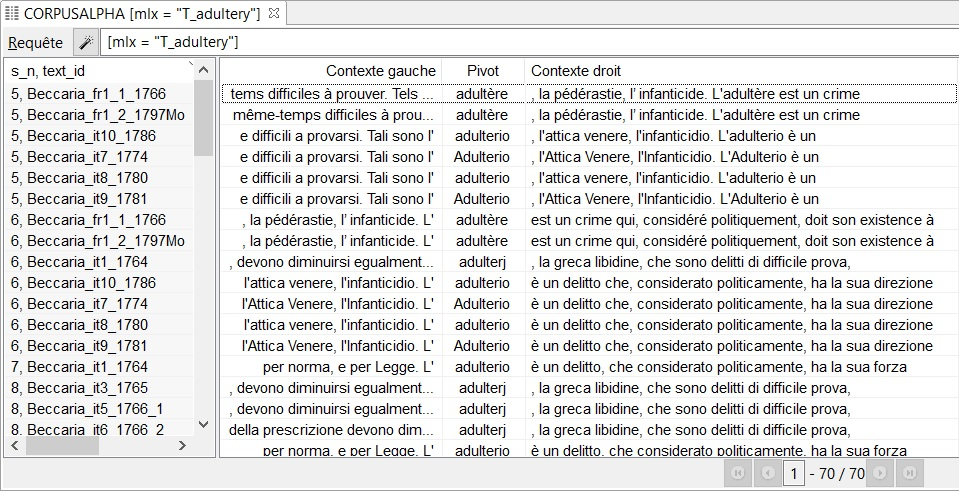
\includegraphics[width=16cm]{Partie3/images/chap2/requete_txm.jpg}
    \label{fig:requete_txm}
\end{figure}

\subsection{Créer les dictionnaires d'annotation}
Après avoir trouvé les identifiants adéquats, nous avons à disposition des listes avec un identifiant pour un mot dans trois langues différentes. L'objectif sera alors de lier ces identifiants à notre corpus pour pouvoir l'analyser et obtenir des statistiques et des données sur le texte\index{Statistique textuelle} sans prendre en compte les distinctions de langues. Pour pouvoir incorporer ces termes et leurs identifiants, il suffit de créer des dictionnaires dans des fichiers Python que nous ajouterons ensuite au texte sous son format \textsc{xml} par la rédaction d'un nouveau script. Deux dictionnaires sont mis en place, un pour chaque type d'identifiant (alphabétique et numérique) et chacun contient tous les mots séparés en trois, à l'aide de variables, que nous appellerons plus tard dans le script. Chacune des variables contient un mini-dictionnaire avec les termes et leurs identifiants pour chaque langue du corpus.

Cependant, un obstacle se présente dans la rédaction de ces dictionnaires, puisqu'un des cas expliqué lors de la présentation des termes est le fait que certaines expressions sont polylexicales, ce qui signifie que dans la mesure où notre annotation se fait dans un texte balisé mot par mot, il sera impossible de mettre l'expression en entier, puisqu'elle ne sera pas retrouvée lors de la lecture du texte et ne sera donc pas annotée. C'est pourquoi les premiers dictionnaires à établir impliquent d'opérer une pré-sélection dans les listes à disposition, avec seulement les expressions monolexicales et leurs identifiants, ce qui réduit la liste des termes. Il est possible de trouver une alternative pour les expressions restantes~: la solution serait alors de choisir un des mots de l'expression et de l'annoter avec l'identifiant. Cela a tout de même une limite dans le cas où l'expression n'aurait pas été écrite de la même façon en fonction des éditions, avec, par exemple, un tiret ou non, ce qui résultera en un balisage différent pour le \textsc{xml} et donc un encodage non complet lors de l'annotation des termes juridiques. De plus, avec un encodage de seulement un des mots, le reste de l'expression sera perdu dans la recherche, à moins de trouver un moyen d'y mettre un attribut à faire ressortir ensuite.

Les dictionnaires seront donc majoritairement composés des expressions monolexicales et par conséquent, le texte ne sera pas entièrement annoté avec le lexique juridique. Pour régler ces problèmes dans nos recherches, il est possible de requêter les expressions manquantes dans les outils à disposition pour exploiter complètement le corpus.

\paragraph{}Une fois les listes de termes juridiques établies et les dictionnaires créés, la dernière étape consiste à rédiger un script pour pouvoir inscrire ces annotations dans le corpus et ensuite procéder à diverses requêtes et extractions de données pour obtenir les informations dont nous avons besoin pour réaliser l'alignement\index{Alignement} recherché.

\section{Procéder à l'annotation~: rédaction et application du script}
L'annotation s'effectue sur un fichier \textsc{xml-tei}, qui a été produit par la plateforme \textsc{txm} lorsque nous avons importé les corpus par langue et à l'aide de son module \emph{TreeTagger}, qui lemmatise chaque forme. L'outil a décomposé le texte par mot, insérant chacun d'eux dans une balise <w>, qui a ensuite été complétée par plusieurs balises et attributs, pour apporter des détails au mot, à savoir sa forme dans le texte, sa catégorie grammatical (POS) et son lemme (LEMMA). Ceci donne une balise mot de ce type~:
\begin{minted}{xml}
<w id="w_beccaria_fr2_1_1773_33" n="33">
<txm:form>ait</txm:form>
<txm:ana resp="#txm" type="#frpos">VER:subp</txm:ana>
<txm:ana resp="#txm" type="#frlemma">avoir</txm:ana>
</w>
\end{minted}
Nous insérons par la suite nous même une forme normalisée, c'est-à-dire la forme modernisée du mot lorsque celui-ci est désuet, forme que nous avions relevé lors de la correction orthographique et de la création du dictionnaire d'enrichissement (voir figure \ref{fig:etape4}). Pour se faire, nous utilisons un script à base d'un dictionnaire et d'expressions régulières ou d'un module \textsc{xml}, effectuant la démarche suivante.
\begin{figure}[H]
    \centering
    \fbox{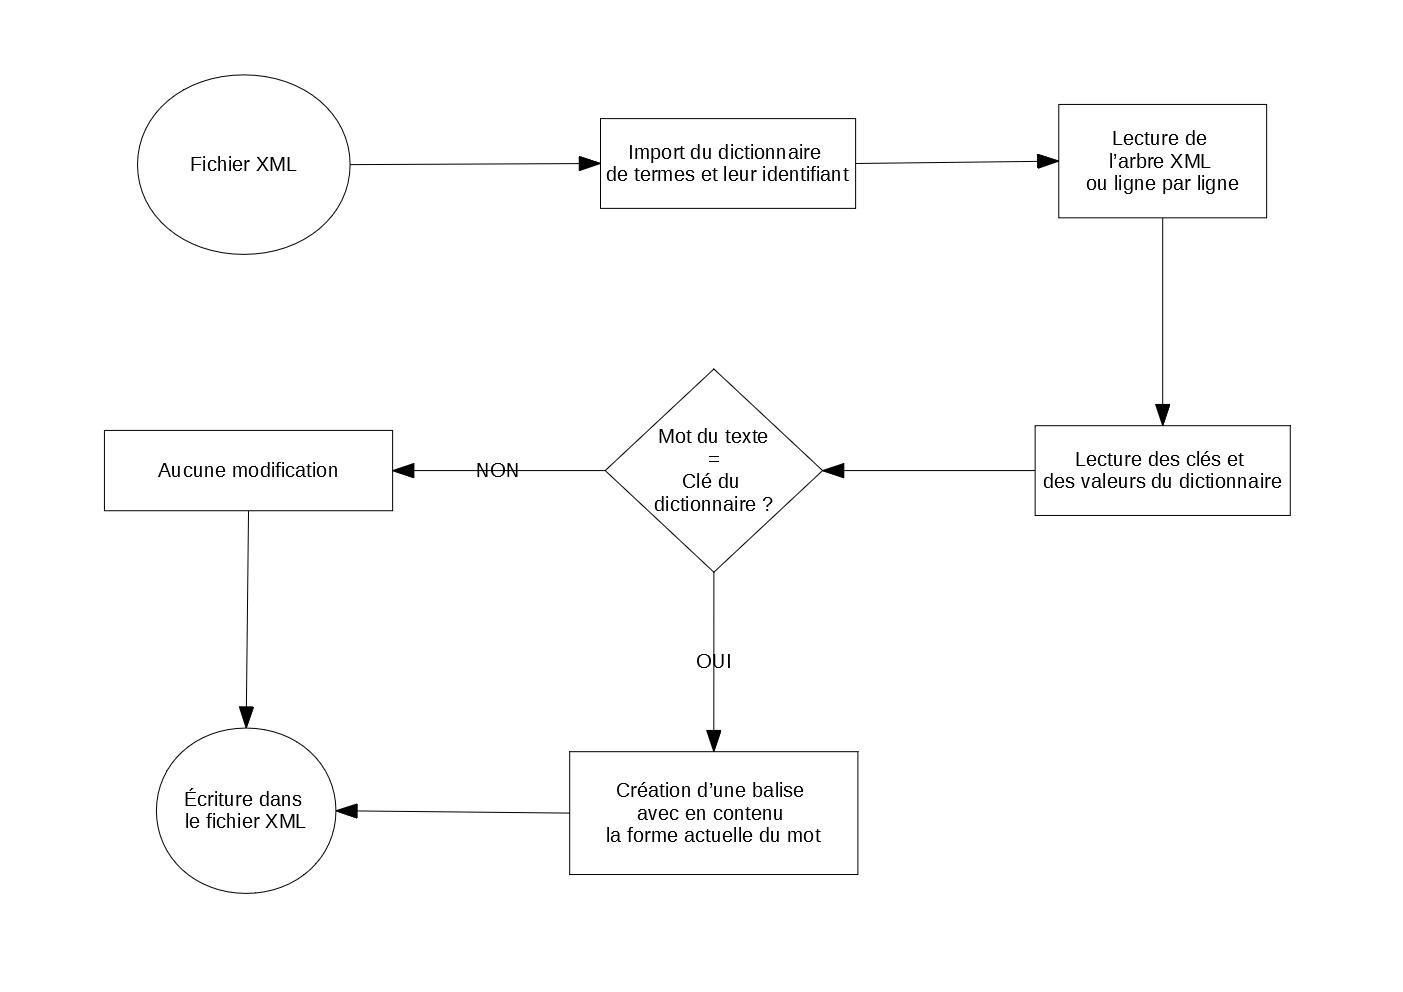
\includegraphics[width=14cm]{Partie3/schemas/normalisation_txm.jpg}}
    \caption{Diagramme d'activité montrant les étapes pour insérer une balise contenant la forme modernisée d'un mot}
    \label{fig:normalisation_txm}
\end{figure}
Partant d'un fichier \textsc{xml}, le processus de la figure \ref{fig:normalisation_txm} consistera à lire le texte et le dictionnaire à disposition, puis lorsque le système trouve un mot correspondant à une des clés du dictionnaire, un nouvel attribut est ajouté à ce mot, dont la valeur est la forme modernisée du mot. 

\paragraph{}À partir de ce fichier \textsc{xml} contenant diverses balises et attributs, nous allons procéder à une annotation en travaillant sur un rajout de balises et un changement de la valeur de l'attribut lorsque le script rencontrera une particularité que nous lui aurons spécifiée. Pour se faire, nous avons à disposition deux scripts, qui effectuent la même tâche mais en utilisant deux techniques différentes, la seconde technique (figure \ref{fig:annotation_xml}) étant une amélioration de la première (figure \ref{fig:annotation_txm}).
\begin{figure}[p]
    \centering
    \fbox{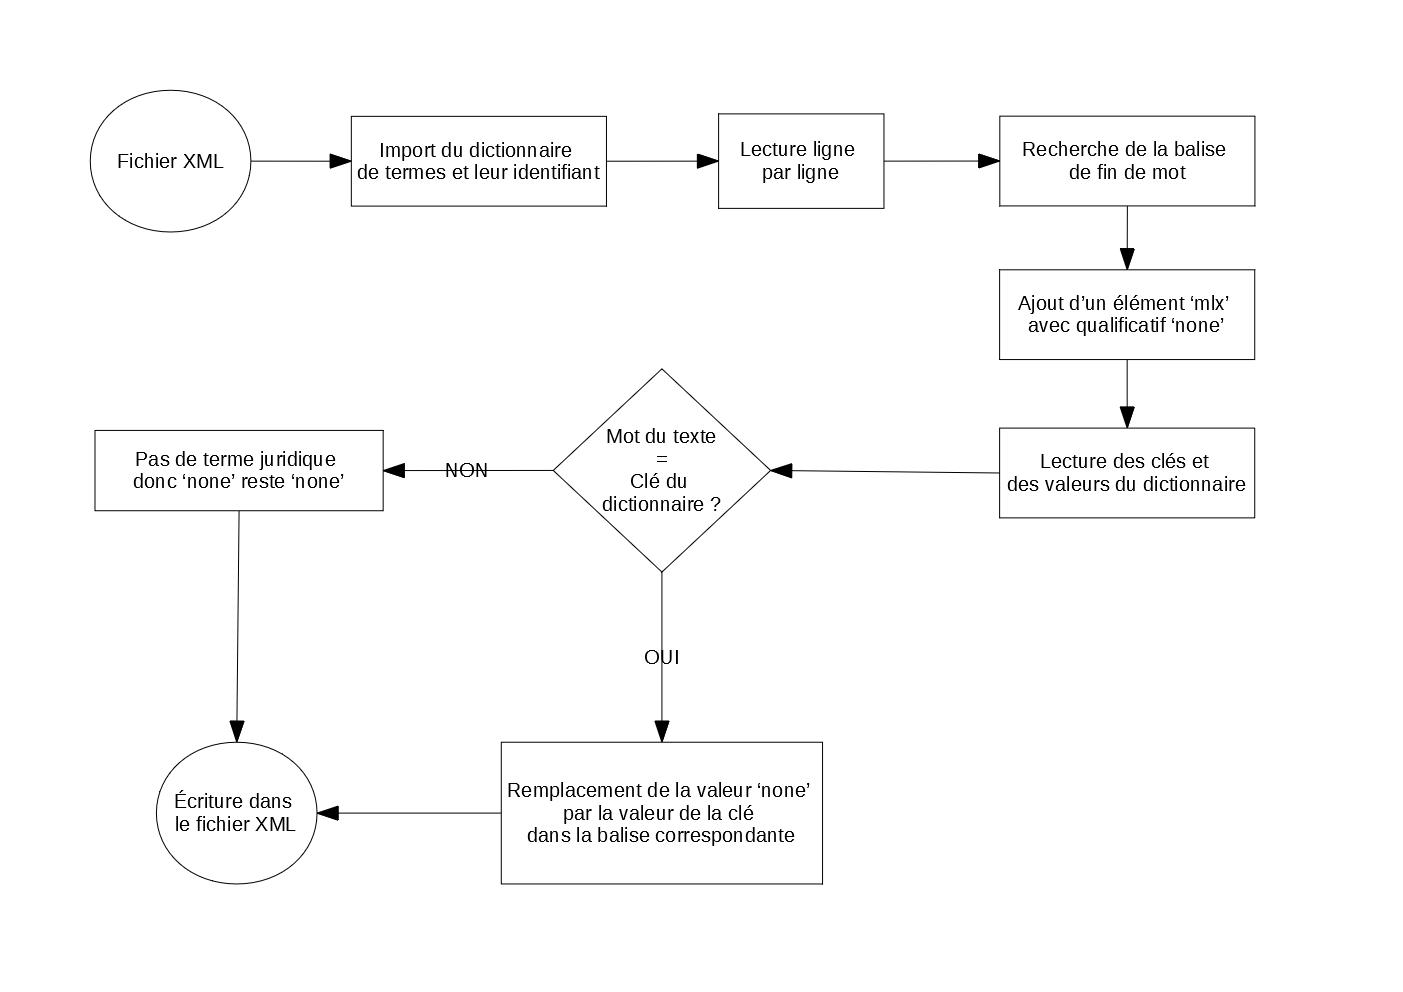
\includegraphics[width=14cm]{Partie3/schemas/annotation_txm.jpg}}
    \caption{Diagramme d'activité représentant les étapes de l'annotation du corpus sous son format \textsc{xml} en utilisant les expressions régulières}
    \label{fig:annotation_txm}
\end{figure}
\begin{figure}[p]
    \centering
    \fbox{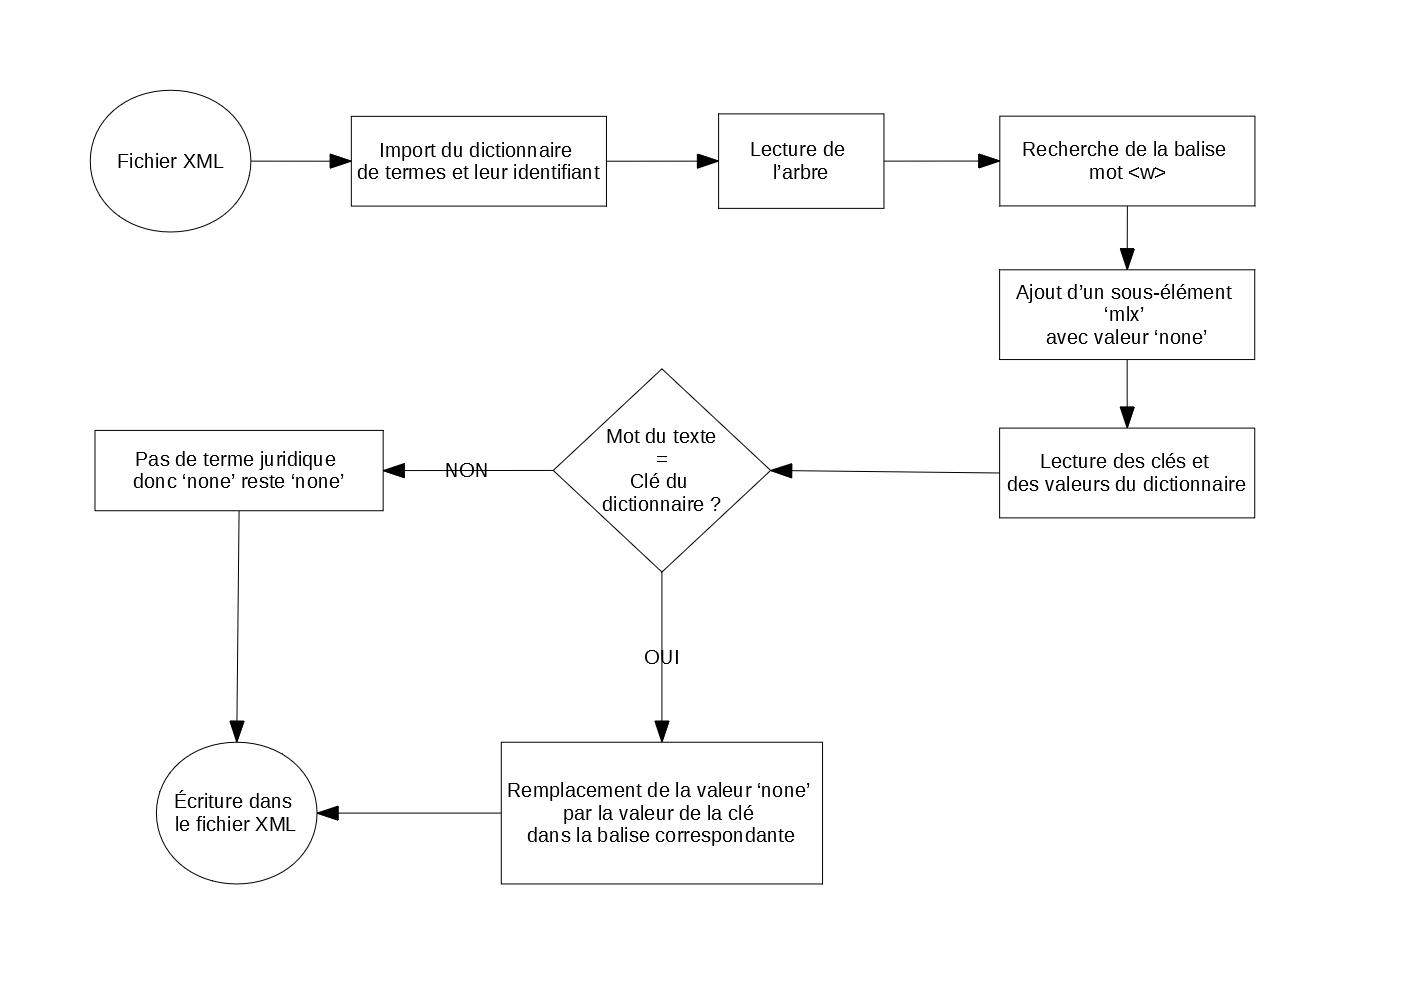
\includegraphics[width=14cm]{Partie3/schemas/annotation_xml.jpg}}
    \caption{Diagramme d'activité représentant les étapes de l'annotation du corpus sous son format \textsc{xml} en utilisant un module \textsc{xml}}
    \label{fig:annotation_xml}
\end{figure}
\paragraph{} Ce processus présente la manière dont, en partant d'un fichier \textsc{xml}, le corpus pourra être annoté des termes juridiques dont nous avons précédemment établi la liste. Dans un premier temps, le processus distribuera un attribut unique à tous les mots présents dans le texte. Dans un second temps, en effectuant à la fois une lecture des balises, de leur texte et du dictionnaire qui lui a été donné, le processus ira lire tous les mots du texte et s'il en trouve un qu'il a déjà rencontré dans le dictionnaire, il changera la valeur du nouvel attribut par la valeur qui correspond à ce qu'il a trouvé dans le dictionnaire. Enfin tout cela est inscrit dans le fichier \textsc{xml}, permettant alors d'avoir un texte annoté suivant ses termes juridiques.

\subsection{Annotations à l'aide d'expressions régulières}
Reposant principalement sur des expressions régulières, le premier script Python comporte trois étapes qui permettent d'insérer les attributs nécessaires au texte pour opérer l'annotation. Tout d'abord, le système récupère le dossier de fichiers que nous lui appelons et le dictionnaire contenu dans la variable demandée dans la requête du terminal. Ensuite, il place, pour tous les mots, juste avant la fermeture de la balise <w> et après la balise du lemme, une nouvelle balise, qui contiendra un attribut de type \textbf{mlx}, qui aura comme valeur unique \og~none~\fg{}. Une fois cela placé, le système ira lire les clés et valeurs contenues dans la variable donnée et en lisant le texte, il cherchera les correspondances aux clés. Dans le cas où il en trouve, ces clés seront contenues dans la balise du lemme et à l'aide d'une expression régulière, il changera la valeur \og~none~\fg{} par la valeur de la clé. Enfin, cela sera écrit dans un nouveau fichier \textsc{xml} contenant ces annotations.

Le positionnement est important dans le texte et dans le script, puisque la liste des termes a été établie de manière à ce que ce soit la forme lemmatisée qui soit rattachée à l'identifiant. Ainsi c'est le lemme qui est recherché dans le fichier \textsc{xml} et non la forme du mot dans le texte. Au final, l'expression régulière s'appuie sur le fait de trouver exactement le lemme dans sa balise correspondante, pour remplacer ensuite la valeur \og~none~\fg{} en la valeur de la clé. Si une balise est insérée entre le lemme et le \textbf{mlx} ou si une modification du texte change la structure du fichier \textsc{xml}, le script ne fonctionnera plus et l'annotation ne pourra pas se faire. Cela représente donc la limite majeure de l'utilisation des expressions régulières dans ce cas. C'est pour cela qu'une autre version a été développée, reposant plus sur le \textsc{xml}, lié avec du Python.

\subsection{Annotations à l'aide d'un module XML}
Python dispose de nombreux modules pour effectuer ce qui lui est demandé et parmi ceux-ci, nous pouvons retrouver un module destiné à l’utilisation de Python pour la manipulation de documents \textsc{xml}~: \emph{ElementTree}\footnote{\url{https://docs.python.org/fr/3/library/xml.etree.elementtree.html}}. Ce dernier se compose de différents éléments pour permettre de manipuler un fichier \textsc{xml}, créer des balises, en supprimer et faire des modifications dans un arbre donné.  Le script à base du module \textsc{xml} suit le même cheminement que le script d’annotations rédigé à l’aide des expressions régulières mais utilise les éléments de \emph{ElementTree}. Par conséquent, après avoir appelé le texte, dont il a lu l’arbre \textsc{xml}, et le dictionnaire associé, ainsi qu’après avoir défini les \textit{namespaces}\footnote{Espace de noms \textsc{xml} qui permet d'employer des éléments et des attributs nommés dans une instance \textsc{xml}} qui se trouvent dans le fichier \textsc{xml}, nous allons chercher, à l’aide d’une boucle, le contenu et les sous-éléments de la balise mot <w>, par le biais de l’élément \textit{iterfind}\footnote{\url{https://docs.python.org/fr/3/library/xml.etree.elementtree.html\#xml.etree.ElementTree.Element.iterfind}}. Nous enrichissons alors cette balise d'un sous élément (\textit{ET.SubElement}\footnote{\url{https://docs.python.org/fr/3/library/xml.etree.elementtree.html\#xml.etree.ElementTree.SubElement}}), pour lequel nous définissons des attributs et une valeur qui sera égale à \og~none~\fg{}. Par la suite, après avoir appelé les clés et valeurs du dictionnaire, le processus consistera à aller chercher dans les valeurs de toutes les balises enfants de <w> (\textit{itertext()}\footnote{\url{https://docs.python.org/fr/3/library/xml.etree.elementtree.html\#xml.etree.ElementTree.Element.itertext}}) ce qui est identique à une des clés du dictionnaire. Lorsque c’est le cas, nous lui faisons simplement changer la valeur \og~none~\fg{} de la balise définie plus tôt. Une fois cela fait, tout est écrit dans l’arbre et le nouveau fichier \textsc{xml} est créé, en contenant les annotations juridiques voulues. 

Cette méthode est plus sûre que la première, car les éléments exacts de l’arbre sont donnés et dans le cas où il y a un changement d’ordre des balises, ce script fonctionnera toujours contrairement au précédent, car il saura exactement quoi aller chercher. La lecture est également plus aisée ici puisque nous lui faisons chercher par balise et par contenu de balise, donc le script est plus simple et plus approprié au texte à disposition.

\paragraph{}Ainsi, à l'aide de l'un ou l'autre des scripts, nous pouvons ajouter les annotations dans le texte sous son format \textsc{xml}, ce qui, couplé avec la balise de normalisation lorsqu'elle est nécessaire, donne un résultat comme cela~:
\begin{minted}{xml}
<w id="w_beccaria_fr2_1_1773_93" n="93">
<txm:form>loix</txm:form>
<txm:ana resp="#txm" type="#norm">lois</txm:ana>
<txm:ana resp="#txm" type="#frpos">NOM</txm:ana>
<txm:ana resp="#txm" type="#frlemma">loi</txm:ana>
<txm:ana resp="#txm" type="#mlx">T_law</txm:ana>
</w>
\end{minted}
Avec cela, nous avons un fichier \textsc{xml-tei} agrémenté, notamment pour que ressorte aisément son lexique juridique, essentiel pour l'étude du texte et l'analyse des différentes versions. En effet, ces annotations nous permettent d'étudier d'une manière différente le texte. Nous avons maintenant la possibilité de travailler le corpus entièrement, sans distinction de langues, puisque l'analyse se basera sur les annotations qui ont un identifiant unique pour les trois versions. En l'état, même si les langues seront différentes, il sera possible d'observer les contextes d'utilisation des termes juridiques, de noter leurs fréquences d'utilisation par année ou par langue et d'effectuer divers autres types d'analyses statistiques\index{Statistique textuelle}, en plus des analyses simples par sous-corpus de langues. Nous pourrons donc procéder à cela et ultérieurement, à partir des données recueillies, obtenir un alignement partiel\index{Alignement!alignement partiel} ciblé\index{Alignement!alignement cible@alignement ciblé} grâce à ce lexique.